%arara : pdflatex
\documentclass[12pt]{article}

\usepackage{../../TP0/style}

\begin{document}
\def\reportnumber{5}
\def\reporttitle{Algorithmes de complexité temporelle linéaire O($a^{n}$) (a$\rangle$1)}
%----------------------------------------------------------------------------------------
%	TITLE PAGE
%----------------------------------------------------------------------------------------


\begin{titlepage} % Suppresses displaying the page number on the title page and the subsequent page counts as page 1
	\newcommand{\HRule}{\rule{\linewidth}{0.5mm}} % Defines a new command for horizontal lines, change thickness here
	
	\center % Centre everything on the page
	
	%------------------------------------------------
	%	Headings
	%------------------------------------------------
	
	\baselineskip=2\baselineskip 
	\textsc{\LARGE Université des Sciences et de la Technologie Houari Boumediene}%\\[1cm] % Main heading such as the name of your university/college

	%------------------------------------------------
	%	Logo
	%------------------------------------------------
	
	%\vfill\vfill
	\vfill
	
\includegraphics[width=0.3\textwidth]{../../TP0/USTHB_Logo.png}\\[1cm] % Include a department/university logo - this will require the graphicx package
	 
	%----------------------------------------------------------------------------------------
	
	\textsc{\Large Conception et Complexité des Algorithme}\\[0.5cm] % Major heading such as course name
	%\textsc{\large Minor Heading}\\[0.5cm] % Minor heading such as course title
	
	%------------------------------------------------
	%	Title
	%------------------------------------------------
	
	\HRule\\[0.4cm]
	\baselineskip=1.2\baselineskip 
	{\huge\bfseries Rapport de Travaux Pratiques N\textdegree  \reportnumber \\ \reporttitle}\\[0.4cm] % Title of your document
	
	\HRule\\[1.5cm]
	
	%------------------------------------------------
	%	Author(s)
	%------------------------------------------------
	
	\begin{minipage}{0.4\textwidth}
		\begin{flushleft}
			\large
			\textit{Binôme}\\
			MOHAMMEDI \textsc{Haroune } % Your name
			\\
			HOUACINE  \textsc{Naila Aziza} % Your name
		\end{flushleft}
	\end{minipage}
	~
	\begin{minipage}{0.4\textwidth}
		\begin{flushright}
			\large
			\textit{Professeur}\\
			Pr. AMANI \textsc{Ferhat} % Supervisor's name
		\end{flushright}
	\end{minipage}
	
	%------------------------------------------------
	%	Date
	%------------------------------------------------
	
	\vfill\vfill\vfill % Position the date 3/4 down the remaining page
	
	{\large\today} % Date, change the \today to a set date if you want to be precise
	
	
	\vfill % Push the date up 1/4 of the remaining page
	
\end{titlepage}


\section{Partie I: Tours de HANOÏ.}

\subsection{Développement de l'algorithme récursif qui résout le problème des "tours de Hanoï". On suppose qu'il y a n disques à transférer (n est un entier naturel, n$\ge$1).}

\begin{sql}

Algorithme Hanoi ;
VAR n, nb : entier ;		
	//n = nombre de disques
  	//nb = nombre de déplacement des disques
  	
DEBUT
    //Partie 1: Lecture des donnees
ecrire("\nDonner le nombre de disques: n = ");			1
lire (n);												2

    //Partie 2: Traitement
nb=0;													3
f_hanoi(n, 1, 3, 2);									4
//appel de la fonction f_hanoi(n, 1, 3, 2)
  
    //Partie 2: Sertie des resultats
ecrire ("le nombre des deplacements nb = ", nb);		5
 
FIN. 
//fin de l`algorithme  Hanoi


//Definition de la fonction f_hanoi
void f_hanoi(int n, int A, int C, int B)
DEBUT 
si (n >= 1)												6 
   	alors debut
	   	f_hanoi(n-1, A, B, C);							7
        printf("\nDéplacer le disque restant de %d vers %d\n", A, B);  											   8
//La tour A devient vide
        nb=nb+1;										9
       f_hanoi(n-1, C, A, B);							10
	fin;
FIN ; 
//fin de la fonction f_hanoi(int n, int A, int C, int B)

 
\end{sql}

\subsection{Complexité:}

\subsubsection{Calcule des complexités temporelles en notation asymptotique de Landau O (Grand O) de  cet  algorithme. }

Soit L le nombre d'instructions de l'algorithme Hanoi (ci-dessus),  fi (i=1…L) la fréquence d'exécution de l'instruction Ii (i=1…L), et F la somme de ces fréquences. \\
On a: L = 10 instructions. \\

 
1- On a pour l'algorithme principal Hanoi : \\
$f_1$=1 ;\\
$f_2$=1 ;\\
$f_3$=1 ;\\
$f_4$=1 + H(n) ; 1 opération pour l'instruction d'appel de la fonction f\_Hanoi(n, 1, 3, 2) \\

H(n) mesure la complexité temporelle de la fonction f\_Hanoi(n, 1, 3, 2)\\
$f_5$=1 ;\\

Donc, F est :\\
F(n)= $\sum_{i=1}^{6}$ $f_i$ = $f_1+f_2+f_3+f_4+f_5 $\\
$\rightarrow$ F(n)=1+1+1+(1 + H(n) )+1\\
$\rightarrow$ F(n)= H(n) +5								(1)\\

2- Pour le calcul de H(n), on procède comme suit :\\
2.1- On calcule les fréquences des instructions de la fonction f\_Hanoi(…) (instructions 6 à 10) :\\

$f_6$=1 ;\\
$f_7$=1 +H(n-1) ;	1 opération pour l'instruction d'appel de la fonction f\_Hanoi(n, A, B, C)\\

H(n-1) mesure la complexité temporelle de la fonction f\_Hanoi(n-1, A, B, C)\\

$f_8$=1 ;\\
$f_9$=2 ;			2 opérations : = et +\\
$f_10$=1 + H(n-1) ;	1 opération pour l'instruction d'appel de la fonction f\_Hanoi(n, C, A, B)\\

H(n-1) mesure la complexité temporelle de la fonction f\_Hanoi(n-1, C, A, B)\\

2.2- On calcule la somme de ces fréquences :\\

H(n)=$\sum_{i=6}^{10}$ $f_i$= $f_6+f_7+f_8+f_9+f_10$  \\
$\rightarrow$ H(n)=1+(1 +H(n-1) )+1+2+(1 +H(n-1) )\\
$\rightarrow$ H(n)=2H(n-1)+6                                 					(2)\\
Et H(0)=1	équation de récurrence \\
si n=0 alors la fonction f\_Hanoi(…) exécute juste le test (n>=1)\\

2.3- On résout l'équation de récurrence (2) avec la méthode de substitution comme suit :\\
H(n)=2H(n-1)+6            \\ 
$\rightarrow$ H(n)=2(2H(n-2)+6)+6   \\          
$\rightarrow$ H(n)=$2^2 H(n-2)+2^1*6+6 $  \\   
$\rightarrow$ H(n)=$2^2 (2H(n-3)+6)+2^1*6+6 $ \\          
$\rightarrow$ H(n)=$2^3 H(n-3)+2^2*6+2^1*6+6 $\\
$\rightarrow$…\\
$\rightarrow$ H(n)=$2^n H(n-n) + 2^(n-1)*6+…+2^1*6+2^0*6$\\
$\rightarrow$ H(n)=$2^n H(0)  + 6(2^(n-1)+…+2^1+2^0)$\\

$\rightarrow$ H(n)=$2^n*1+6((2^n-1)/(2-1))=2^n+6(2^n-1)=[7*2]^n-6	$		(3)\\
La relation (3) représente la solution en notation exacte de l'équation de récurrence (2).\\

On montre aisément que :\\
H(n)= $7*2^n-6$       \\
$\rightarrow$ H(n)$\le 7*2^n-6+6=7*2^n$\\
$\rightarrow$ H(n)=O($2^n$)       \\          							(4)\\
H(n) en notation asymptotique\\

On conclut alors que la fonction f\_Hanoi(…) a une complexité temporelle exponentielle.\\

3- On calcule enfin la fonction F(n) en y remplaçant la solution H(n) dans la relation (1) :\\
F(n)= H(n) +5\\
$\rightarrow$ F(n)=$(7*2^n-6)+5= 7*2^n-1$         					(5)\\
F(n) en notation exacte\\

On montre aisément aussi que :\\
F(n)=$ 7*2^n-1$       \\
$\rightarrow$ F(n)$\le 7*2^n-6+1= 7*2^n$\\
$\rightarrow$ F(n)=O($2^n$)                 							(6)\\
F(n) en notation asymptotique\\

On conclut là aussi que l'Algorithme du problème des « tours de Hanoi » a une complexité temporelle exponentielle.\\

En conséquence, la complexité temporelle CT de l'algorithme Hanoi est: \\

  \[ 
\left\{
\begin{array}{r c l}
CT(n)=F(n)=7*2^n-1 \quad \quad \quad \quad \quad en notation exacte\\
CT(n)=F(n)= O(2^n)\quad \quad \quad en notation asymptotique
\end{array}
\right.
\]
\\




\subsubsection{Calculer la complexité spatiale en notation exacte et en notation asymptotique de Landau O (Grand O) de  cet  algorithme notée s(n).}
 
1- On a pour l'algorithme principal Hanoi : \\
n et nb : deux (2) variables de type entier
correspondant à 8 octets au totale 

H(n) mesure la complexité spatiale de la fonction f\_Hanoi(n, 1, 3, 2)\\

Donc, F est :\\
F(n)= H(n) + 2	$\quad \quad \quad $		(1)\\

2- Pour le calcul de H(n), on procède comme suit :\\
2.1- On calcule les fréquences des transfère de disque de la fonction f\_Hanoi(…) :\\

Tel que on alloue 2*2 + 1 case pour n = 2 disques\\
donc $2^2$+(2-1)

2.2- On calcule la somme de ces allocations :\\

Et H(0)=2	équation de récurrence \\
si n=0 alors la fonction f\_Hanoi(…) exécute juste le test (n$\ge$1)\\

2.3- On résout l'équation de récurrence (2) avec la méthode de substitution comme suit :\\
H(n)=2(H(n-1))+n           \\ 
$\rightarrow$ H(n)=2(2(H(n-2))+n )+n   \\          
$\rightarrow$ H(n)=$2^2 H(n-2)+2^1*n+n $  \\   
$\rightarrow$ H(n)=$2^2 (2H(n-3)+n)+2^1*n+n $ \\          
$\rightarrow$ H(n)=$2^3 H(n-3)+2^2*n+2^1*n+n $\\
$\rightarrow$…\\
$\rightarrow$ H(n)=$2^n H(n-n) + 2^(n-1)*n+…+2^1*n+2^0*n$\\
$\rightarrow$ H(n)=$2^n H(0)  + n(2^(n-1)+…+2^1+2^0)$\\

$\rightarrow$ H(n)=$2^n*1+n((2^n-1)/(2-1))=2^n+n(2^n-1)= [7*2]^n-n	$		(3)\\
La relation (3) représente la solution en notation exacte de l'équation de récurrence (2).\\

On montre aisément que :\\
H(n)= $7*2^n-n$       \\
$\rightarrow$ n $\le 7*2^n $\\
$\rightarrow$ H(n)=O($2^n$)       \\          							(4)\\
H(n) en notation asymptotique\\

On conclut alors que la fonction f\_Hanoi(…) a une complexité temporelle exponentielle.\\

3- On calcule enfin la fonction F(n) en y remplaçant la solution H(n) dans la relation (1) :\\
F(n)= H(n) + 2\\
$\rightarrow$ F(n)=$(7*2^n-n)+2= 7*2^n-n+2$         					(5)\\
F(n) en notation exacte\\

On obtiens ainsi :\\
$\rightarrow$ F(n)=O($2^n$)                 							(6)\\
F(n) en notation asymptotique\\

On conclut là aussi que l'Algorithme du problème des « tours de Hanoi » a une complexité spatiale exponentielle.\\

En conséquence, la complexité spatiale CS de l'algorithme Hanoi est: \\

  \[ 
\left\{
\begin{array}{r c l}
CS(n)=F(n)=7*2^n-n+2 \quad \quad \quad \quad \quad en notation exacte\\
CS(n)=F(n)= O(2^n)\quad \quad \quad en notation asymptotique
\end{array}
\right.
\]
\\



\subsection{Développement de programme correspondant avec le langage C.}
\subsubsection{Programme principale}
\begin{sql}
#include <stdlib.h>
#include <stdio.h>

//Déclaration de la fonction hanoi
void hanoi(int, int, int, int);
int nb;				
//nb est une variable globale

int main(void)
{
  int n;				
  //n = nombre de disques
  //nb = nombre de déplacement des disques
  clock_t t1, t2;		
  //clock_t désigne le type temps
  double delta;			
  //delta mesure la durée d`exécution du programme entre les points t1 et t2
  
  //Partie 1: Lecture des données
  printf("\nDonner le nombre de disques: n = ");
  scanf("%d", &n);
				
  //Partie 2: Traitement
  nb=0;
  t1=clock();			

  hanoi(n, 1, 3, 2);          	
  //appel de la fonction hanoi(n, 1, 3, 2)
  //On suppose : A=1, B=2 et C=3
  
  t2=clock();			

  delta=(double)(t2-t1)/CLOCKS_PER_SEC;	  
  printf("\n\n nb=%d déplacements", nb);
  printf("\n\nEntrer une touche quelconque pour terminer le programme: ");
  getchar(); getchar();
  return(0);
}
//fin du programme
\end{sql}

\subsubsection{Fonction Hanoi}

\begin{sql}

//Définition de la fonction hanoi
void hanoi(int n, int A, int C, int B)
{
  if (n >= 1) 
    {
        hanoi(n-1, A, B, C);
        printf("\nDéplacer le disque restant de %d vers %d\n", A, B);  
        //La tour A devient vide
        nb=nb+1;		
        //Lors des mesures du temps, ces 2 instructions doivent etre bloquees (par exemple mises en commentaires)
        hanoi(n-1, C, A, B);
    }
}
//fin de la fonction hanoi

\end{sql}



\subsubsection{Résultat}
\begin{sql}
Donner le nombre de disques: n = 2
Deplacer le disque restant de 1 vers 3
Deplacer le disque restant de 1 vers 2
Deplacer le disque restant de 2 vers 3

 nb=3 deplacements


Donner le nombre de disques: n = 3
Deplacer le disque restant de 1 vers 3
Deplacer le disque restant de 1 vers 2
Deplacer le disque restant de 3 vers 2
Deplacer le disque restant de 1 vers 3
Deplacer le disque restant de 2 vers 1
Deplacer le disque restant de 2 vers 3
Deplacer le disque restant de 1 vers 3

 nb=7 deplacements
 
 ...
\end{sql}

\subsection{Mesure des temps d'exécution.}
Grâce à l'exécution du programme C vu précédemment nous avons obtenu les temps d'exécution suivants.

\subsubsection{Remplissage du tableau:}
\color{blue}

\begin{tabular}{|p{3cm}||p{1.7cm}|p{1.7cm}|p{1.7cm}|p{1.7cm}|p{1.7cm}|p{1.7cm}|p{1.7cm}|}
\hline
Nombre de disque (N) : & $\le 4 $ & 5 & 6 & 7 & 8 & 9 & 10  \\
\hline
Temps d'exécution : & 0.000001 & 0.000002 & 0.000002 & 0.000004 & 0.000006 & 0.000022  & 0.000022\\
\hline

\end{tabular}
\\

\begin{tabular}{|p{3cm}||p{1.7cm}|p{1.7cm}|p{1.7cm}|p{1.7cm}|p{1.7cm}|p{1.7cm}|p{1.7cm}|}
\hline
Nombre de disque (N) : & 11 & 12 & 13 & 14 & 15 & 16 & 17  \\
\hline
Temps d'exécution :  & 0.000038 & 0.000089 & 0.000191 & 0.000371 & 0.000730 & 0.001448 & 0.002859 \\
\hline

\end{tabular}
\\

\begin{tabular}{|p{3cm}||p{1.7cm}|p{1.7cm}|p{1.7cm}|p{1.7cm}|p{1.7cm}|p{1.7cm}|p{1.7cm}|}
\hline
Nombre de disque (N) : & 18 & 19 & 20 & 21 & 22 & 23 & 24  \\
\hline
Temps d'exécution :  & 0.004113 & 0.003898 & 0.008290 & 0.016846 & 0.033388 & 0.075825 & 0.121189  \\
\hline

\end{tabular}
\\

\begin{tabular}{|p{3cm}||p{1.7cm}|p{1.7cm}|p{1.7cm}|p{1.7cm}|p{1.7cm}|p{1.7cm}|p{1.7cm}|}
\hline
Nombre de disque (N) : & 25 & 26 & 27 & 28 & 29 & 30 & 31  \\
\hline
Temps d'exécution : & 0.241212 & 0.488855 & 0.981898 & 1.954524 & 4.279422 & 9.125135 & 17.255445  \\
\hline

\end{tabular}
\\

\begin{tabular}{|p{3cm}||p{1.7cm}|p{1.7cm}|p{1.7cm}|p{1.7cm}|p{1.7cm}|p{1.7cm}|p{1.7cm}|}
\hline
Nombre de disque (N) : & 32 & 33 & 34 & 35 & ... & ... & 64 \\
\hline
Temps d'exécution : & 34.634779 & 64.643997 & 132.495650 & 263.460620 &  &  & \\
\hline

\end{tabular}
\\

 


\textrm{  }
\\
\color{black}





\subsection{Représentation par un graphe, Gf(n) les variations de la fonction de la complexité temporelle théorique  fonction de n; et par un (1) autre graphe,  les variations  du temps d'exécution T(n) en fonction de n.}
\texttt{  }\\

\subsubsection{Représentation des graphes de la variation du temps d'exécution :}


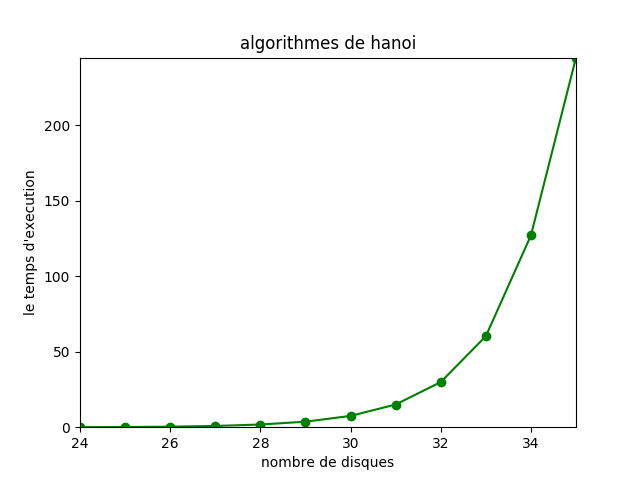
\includegraphics[width=1\textwidth]{graphe/hanoi.png}

\subsubsection{Représentation du graphe Gf de la complexité théorique :}

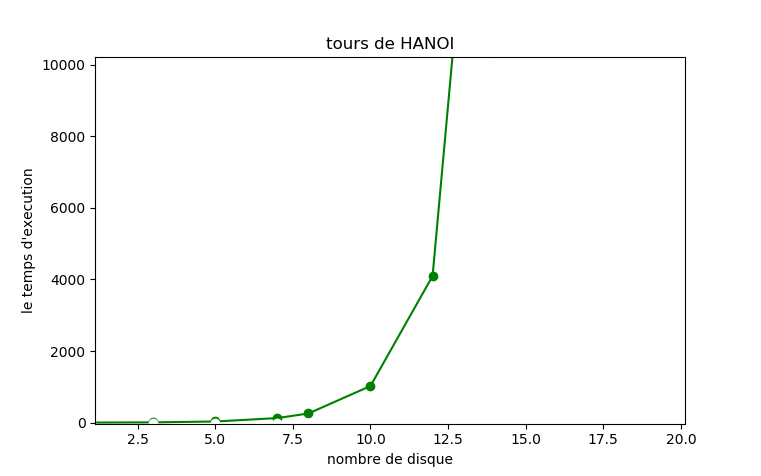
\includegraphics[width=1\textwidth]{graphe/THhanoi.png}


\subsection{Interprétation des résultats.}
\subsubsection{Comparaison des mesures de temps d'exécution avec le pire et meilleur cas:}
	  
Vu que ici nous n'avons pas complexité au pire et meilleur cas , nous comparons alors la complexité exacte obtenu : il nous parait claire de part le graphe que les temps d'exécutions suivent la même évolution, en O($2^n$).

\subsubsection{Remarque et déduction d'une fonction T(n) reliant n au temps d'exécution.}

On remarque que les temps d'exécution sont approximativement multipliés par 2 lorsque N est incrémenté de 1.
\\

\color{blue}
Exemples:
\color{black} 
\\
N1 = $6  \Rightarrow  $  T1 = 0.000002
\\
N2 = $7 \approx N1 + 1  \Rightarrow  $  T2 = 0.000004 $\approx 2 * T1 $
\\

Aussi
\\
N1 = $12 \Rightarrow $  T1 = 0.000089
\\
N2 = $13 \approx N1 + 1 \Rightarrow $  T2 = 0.000191 $\approx 2 * T1 $
\\

On en déduit que le temps d'exécution est proportionnel à N, ce que l'on peut représenter par la formule suivante
: 
\begin{center}
\color{red}
	$T(N+1) = 2^1 *T(N)$ pour tous $ N \in [0 - 64] $	
	
\color{black}
(x étant la tangente d'un point sur le graphe).
\end{center}

Nous ne pouvant pas généraliser car les testes que nous avons fait n'englobent pas toutes les valeurs possibles, 
	



\subsubsection{Comparaison de la complexité théorique et expérimentale. }
Dans le cas des données de l'échantillon la complexité théorique et expérimentale sont du même ordre de grandeur que la complexité théorique,\\
\color{blue}
Donc Le modèle théorique est conforme aux mesures expérimentales.
\color{black}
\\


\end{document}